\documentclass[a4paper,11pt]{article}
\usepackage{amsmath,amsthm,amsfonts,amssymb,amscd,amstext,vmargin,graphics,graphicx,tabularx,multicol} \usepackage[french]{babel}
\usepackage[utf8]{inputenc}  
\usepackage[T1]{fontenc} 
\usepackage[T1]{fontenc}
\usepackage{amsmath,amssymb}
\usepackage{pstricks-add,tikz,tkz-tab,variations}
\usepackage[autolanguage,np]{numprint} 
\usepackage{color}
\usepackage{ulem}

\setmarginsrb{1.5cm}{0.5cm}{1cm}{0.5cm}{0cm}{0cm}{0cm}{0cm} %Gauche, haut, droite, haut
\newcounter{numexo}
\newcommand{\exo}[1]{\stepcounter{numexo}\noindent{\bf Exercice~\thenumexo} : \marginpar{\hfill /#1}}
\reversemarginpar


\newcounter{enumtabi}
\newcounter{enumtaba}
\newcommand{\q}{\stepcounter{enumtabi} \theenumtabi.  }
\newcommand{\qa}{\stepcounter{enumtaba} (\alph{enumtaba}) }
\newcommand{\initq}{\setcounter{enumtabi}{0}}
\newcommand{\initqa}{\setcounter{enumtaba}{0}}

\newcommand{\be}{\begin{enumerate}}
\newcommand{\ee}{\end{enumerate}}
\newcommand{\bi}{\begin{itemize}}
\newcommand{\ei}{\end{itemize}}
\newcommand{\bp}{\begin{pspicture*}}
\newcommand{\ep}{\end{pspicture*}}
\newcommand{\bt}{\begin{tabular}}
\newcommand{\et}{\end{tabular}}
\renewcommand{\tabularxcolumn}[1]{>{\centering}m{#1}} %(colonne m{} centrée, au lieu de p par défault) 
\newcommand{\tnl}{\tabularnewline}

\newcommand{\trait}{\noindent \rule{\linewidth}{0.2mm}}
\newcommand{\hs}[1]{\hspace{#1}}
\newcommand{\vs}[1]{\vspace{#1}}

\newcommand{\N}{\mathbb{N}}
\newcommand{\Z}{\mathbb{Z}}
\newcommand{\R}{\mathbb{R}}
\newcommand{\C}{\mathbb{C}}
\newcommand{\Dcal}{\mathcal{D}}
\newcommand{\Ccal}{\mathcal{C}}
\newcommand{\mc}{\mathcal}

\newcommand{\vect}[1]{\overrightarrow{#1}}
\newcommand{\ds}{\displaystyle}
\newcommand{\eq}{\quad \Leftrightarrow \quad}
\newcommand{\vecti}{\vec{\imath}}
\newcommand{\vectj}{\vec{\jmath}}
\newcommand{\Oij}{(O;\vec{\imath}, \vec{\jmath})}
\newcommand{\OIJ}{(O;I,J)}

\newcommand{\bmul}[1]{\begin{multicols}{#1}}
\newcommand{\emul}{\end{multicols}}


\newcommand{\reponse}[1][1]{%
\multido{}{#1}{\makebox[\linewidth]{\rule[0pt]{0pt}{20pt}\dotfill}
}}

\newcommand{\titre}[5] 
% #1: titre #2: haut gauche #3: bas gauche #4: haut droite #5: bas droite
{
\noindent #2 \hfill #4 \\
#3 \hfill #5

\vspace{-1.6cm}

\begin{center}\rule{6cm}{0.5mm}\end{center}
\vspace{0.2cm}
\begin{center}{\large{\textbf{#1}}}\end{center}
\begin{center}\rule{6cm}{0.5mm}\end{center}
}



\begin{document}
\pagestyle{empty}
\titre{Correction contrôle 3 : Transformations et homothétie}{Nom}{Prénom}{Date}{Classe}


\exo{4}


\noindent \q  L'image  du  triangle  1  par  la  symétrie axiale d'axe \red (xy)\black est \red le triangle 3 \black .\\
\q  L'image  du  triangle  1  par  la  symétrie centrale de centre \red A \black est \red le triangle 5 \black .\\
\q L'image du triangle 1 par la translation de vecteur \red $\vec{EF}$ est le triangle 2 \black \\
\q Le triangle 1 a pour image le triangle 4 par la rotation de centre \red A et d'angle 90 \degre \black(le sens   de   la   rotation   est   indiqué   par   la flèche).\\



\exo{5}

\includegraphics[scale=0.85]{correctionexo2controle.eps} 




\exo{2}

\hspace*{1cm} 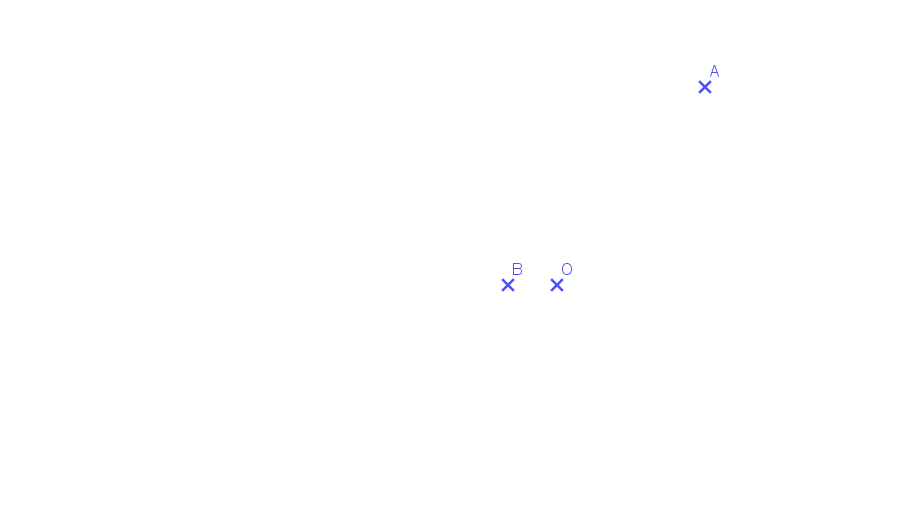
\includegraphics[scale=1]{exohomo1.eps} 

\noindent \initq \q Placer le point B' image du point B par l'homothétie de centre O et de rapport k = 7.\\
\q Placer le point A' image du point A par l'homothétie de centre O et de rapport k = -0,6.\\


\exo{2} Tracer $F_{2}$ l'image de la figure $F_{1}$ par l'homothétie de centre L et de rapport k = 0,5.


\begin{flushleft}
\includegraphics[scale=0.75]{correctionexo5.eps} 
\end{flushleft}


\exo{3}\\

\initq \q \includegraphics[scale=0.8]{correctionexo6a.eps} \\


\q \includegraphics[scale=0.8]{correctionexo6b.eps} 

\exo{2,5}
Soit MONA un rectangle de longueur 12 m et de largeur 5 m et M'O'N'A' son image par une homothétie de rapport k = 6.\\
\red
\initq \q  On sait que MONA est un rectangle, ainsi $\mathcal{A}_{MONA}= l \times L$ \hspace*{0.5cm} $\mathcal{A}_{MONA}= 12 \times 5 = 60 m^{2}$ \\

\black
\red \q Comme M'O'N'A' est l'image de MONA par une homothétie de rapport k=6, d'après la propriété sur les longueurs, les longueurs du rectangle M'O'N'A' sont celles du rectangle MONA multiplié par k (ici k=6). Et l'aire est multipliée par $k^{2}.$\hspace*{1.5cm} Soit $\mathcal{A}_{M'O'N'A'}=k^{2} \times \mathcal{A}_{MONA}$ \hspace*{0.5cm}  \\
$\mathcal{A}_{M'O'N'A'}=6^{2} \times \mathcal{A}_{MONA}$ \hspace*{0.5cm} $\mathcal{A}_{M'O'N'A'}=36 \times \mathcal{A}_{MONA}$ \hspace*{0.5cm} $\mathcal{A}_{M'O'N'A'}=2 160 m^{2}$




\end{document}
